% Этот шаблон документа разработан в 2014 году
% Данилом Фёдоровых (danil@fedorovykh.ru) 
% для использования в курсе 
% <<Документы и презентации в \LaTeX>>, записанном НИУ ВШЭ
% для Coursera.org: http://coursera.org/course/latex .
% Исходная версия шаблона --- 
% https://www.writelatex.com/coursera/latex/3.2

\documentclass[a4paper,12pt]{article}

%%% Работа с русским языком
\usepackage{cmap}					% поиск в PDF
\usepackage{mathtext} 				% русские буквы в формулах
\usepackage[T2A]{fontenc}			% кодировка
\usepackage[utf8]{inputenc}			% кодировка исходного текста
\usepackage[english,russian]{babel}	% локализация и переносы

%%% Дополнительная работа с математикой
\usepackage{amsmath,amsfonts,amssymb,amsthm,mathtools} % AMS
\usepackage{icomma} % "Умная" запятая: $0,2$ --- число, $0, 2$ --- перечисление

%% Номера формул
\mathtoolsset{showonlyrefs=true} % Показывать номера только у тех формул, на которые есть \eqref{} в тексте.
%\usepackage{leqno} % Нумерация формул слева

%%New Commands
\newcommand{\norm}[1]{\left\lVert#1\right\rVert}





%% Свои команды
\DeclareMathOperator{\sgn}{\mathop{sgn}}

%% Перенос знаков в формулах (по Львовскому)
\newcommand*{\hm}[1]{#1\nobreak\discretionary{}
{\hbox{$\mathsurround=0pt #1$}}{}}

%%% Работа с картинками
\usepackage{graphicx}  % Для вставки рисунков
\graphicspath{{images/}{images2/}}  % папки с картинками
\setlength\fboxsep{3pt} % Отступ рамки \fbox{} от рисунка
\setlength\fboxrule{1pt} % Толщина линий рамки \fbox{}
\usepackage{wrapfig} % Обтекание рисунков текстом

%%% Работа с таблицами
\usepackage{array,tabularx,tabulary,booktabs} % Дополнительная работа с таблицами
\usepackage{longtable}  % Длинные таблицы
\usepackage{multirow} % Слияние строк в таблице

%%% Теоремы
\theoremstyle{plain} % Это стиль по умолчанию, его можно не переопределять.
\newtheorem{definition}{Definition}[section]


 
\theoremstyle{remark} % "Примечание"
\newtheorem*{nonum}{Решение}

%%% Программирование
\usepackage{etoolbox} % логические операторы

%%% Страница
%\usepackage{extsizes} % Возможность сделать 14-й шрифт
\usepackage{geometry} % Простой способ задавать поля
	\geometry{top=25mm}
	\geometry{bottom=35mm}
	\geometry{left=35mm}
	\geometry{right=20mm}
 %
%\usepackage{fancyhdr} % Колонтитулы
% 	\pagestyle{fancy}
% 	\renewcommand{\headrulewidth}{0mm}  % Толщина линейки, отчеркивающей верхний колонтитул
 %	\lfoot{Нижний левый}
 %	\rfoot{Нижний правый}
 %	\rhead{Верхний правый}
 %	\chead{Верхний в центре}
 %	\lhead{Верхний левый}
 % \cfoot{Нижний в центре} % По умолчанию здесь номер страницы

\usepackage{setspace} % Интерлиньяж
%\onehalfspacing % Интерлиньяж 1.5
%\doublespacing % Интерлиньяж 2
%\singlespacing % Интерлиньяж 1

\usepackage{lastpage} % Узнать, сколько всего страниц в документе.

\usepackage{soul} % Модификаторы начертания

\usepackage{hyperref}



%\renewcommand{\familydefault}{\sfdefault} % Начертание шрифта

\usepackage{multicol} % Несколько колонок

\author{Барсегян Сергей}
\title{Вычислительная математика։ Распространение возмущения в изотропной среде}
\date{\today}

\begin{document} % конец преамбулы, начало документа
\maketitle

\begin{abstract}
	Решается волновое уравнение для изотропной среды с вейвлетным возмущением в центре рассчётной сетки. Уравнение решается методом конечных разностей и псевдоспектральным методом. Проводится анализ Неймана для выявления анизотропии метода конечных разностей. Строится диаграмма направлений для метода конечных разностей. 
\end{abstract}

\section{Теория}

$$
\partial_{t}^{2} p(x, z, t)=c^{2}\left[\partial_{x}^{2} p(x, z, t)+\partial_{z}^{2}p(x, z, t)\right]+s(x, z, t)
$$
$$
P(r, t)=\frac{1}{2 \pi c^{2}} \frac{H\left(t-\frac{|r|}{c}\right)}{\sqrt{t^{2}-\frac{r^{2}}{c^{2}}}}
$$

$$
p(x, z, t) \quad \rightarrow \quad p_{j, k}^{n}=p(j d x, k d z, n d t)
$$

$$
s ( x , z , t ) \quad \rightarrow \quad s _ { j k k } ^ { n } = s ( j d x , k d z , n d t )
$$

$$d z = d x
$$



\section{Анализ Неймана}

$$
p_{j,k}^{n} = e^{i\left(k_{x}j d x + k_{z}kdx - \omega ndt \right)}$$
	


\begin{figure}
	\centering
	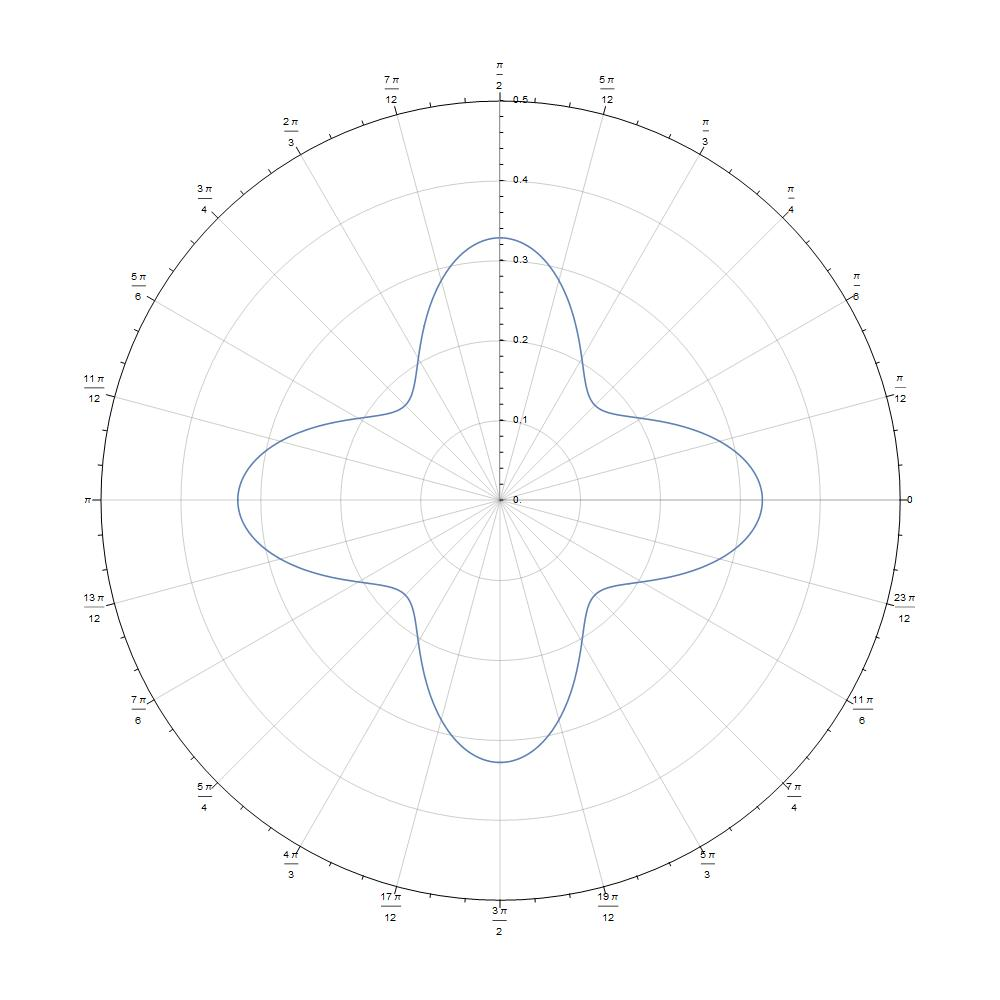
\includegraphics[width=0.7\linewidth]{screenshot003}
	\caption{Дисперсионная диаграмма для конечно-разностного метода}
	\label{fig:screenshot003}
\end{figure}


$$
\frac{p_{j, k}^{n+1}-2 p_{j, k}^{n}+p_{j, k}^{n-1}}{d t^{2}}=c_{j}^{2}\left(\partial_{x}^{2} p+\partial_{z}^{2} p\right)+s_{j, k}^{n}
$$


$$
\begin{aligned} \partial_{x}^{2} p &=\frac{p_{j+1, k}^{n}-2 p_{j, k}^{n}+p_{j-1, k}^{n}}{d x^{2}} \\ \partial_{z}^{2} p &=\frac{p_{j, k+1}^{n}-2 p_{j, k}^{n}+p_{j, k-1}^{n}}{d z^{2}} \end{aligned}
$$


$$
c^{n u m}\left(k_{x} , k_{z}\right)=\frac{2}{k d t} \sin ^{-1}\left[\sqrt{\frac{d t^{2}}{d x^{2}} c^{2}\left(\sin \left(\frac{k_{x} d x}{2}\right)^2+\sin \left(\frac{k_{2} d x}{2}\right)^2\right)}\right]
$$

\end{document} % конец документа

